Di seguito si introducono alcuni concetti 
per permettere al lettore di acquisire le nozioni necessarie alla
corretta fruizione del materiale successivo.

\section{Funzioni di hash}
\label{sub:hash}
Una \textbf{funzione di hashing}~\cite{hash} \(h\) è una funzione che permette di associare,
a una qualsiasi sequenza \(m\) di lunghezza arbitraria in input, una sequenza
in output \(h(m)\) di lunghezza costante. 
Questo valore restituito in output è chiamato valore di hash, stringa di hash,
o anche semplicemente \textbf{hash}, mentre il valore preso in input è detto
\textbf{preimmagine}. Possiamo pensare a questa funzione come una ``macchina per
impronte digitali", per ogni sequenza in input essa riesce a calcolarne una stringa binaria
che la identifica univocamente.

Una funzione di hash ha tre caratteristiche fondamentali:
innanzitutto è \emph{deterministica}, ciò significa che per lo stesso input essa deve
generare sempre lo stesso output, deve poi generare esclusivamente
\emph{sequenze in output con una lunghezza fissa}, ciò significa che per qualsiasi input
di qualsiasi lunghezza il risultato dovrà avere sempre una lunghezza di \(b\) bit decisa
a priori, infine deve essere \emph{uniforme}, ovvero i suoi output devono essere
uniformemente distribuiti nel codominio della funzione.
Una stringa di hash, essendo una sequenza binaria, può essere rappresentata in molti modi,
nell'ambito di questo documento presenteremo i vari hash come stringhe esadecimali.

Mentre una funzione di hash generica è tranquillamente utilizzabile per contesti
in cui non è necessaria una particolare sicurezza nel proteggere le caratteristiche
delle preimmagine, quando si ha bisogno che le
informazioni in input rimangano nascoste e si necessita di una maggior sicurezza a scapito
della velocità si ricorre alle \textbf{funzioni crittografiche di hash}.

Una funzione crittografica di hash ha le stesse caratteristiche di una funzione di
hash normale ma aggiunge delle proprietà che deve seguire per poter essere considerata
\emph{crittograficamente sicura}, i valori della sua lunghezza b sono tipicamente
128, 256 e 512, si va quindi ad ottenere degli output potenzialmente molto più lunghi
e che non sembrano adatti alle implementazioni all'interno di semplici strutture dati
per cui le classiche funzioni di hash sono designate.

Le proprietà che permettono di definire una funzione crittografica di hash come sicura sono:
\begin{enumerate}
    \item \emph{Resistenza alla preimmagine}: Dato un hash \(h\) deve essere difficile riuscire a
    trovare un input \(m\) tale che \(h = h(m)\).
    \item \emph{Resistenza alla seconda preimmagine}: Dato un input \(m_1\) deve essere difficile
    riuscire a trovare un diverso input \(m_2\) tale che \(h(m_1) = h(m_2)\).
    \item \emph{Resistenza alla collisione}: Dati due messaggi \(m_1\) ed \(m_2\), deve essere
    difficile che i due messaggi abbiano lo stesso hash, quindi con \(h(m_1) = h(m_2)\).
\end{enumerate}
Da quanto detto si evince che una funzione crittografica di
hash effettua un'operazione unidirezionale: non è possibile (o perlomeno non dovrebbe esserlo),
partendo dal singolo hash, risalire alla preimmagine. \\
Per riuscire a mantenere tali proprietà la funzione, durante la fase di generazione
dell'output, effettua diverse e differenti operazioni sulla preimmagine
che fanno si che anche un solo minuscolo cambiamento all'input generi
un \emph{effetto valanga} sull'output, cambiando radicalmente, se non completamente,
l'hash generato.

Le funzioni crittografiche di hash vengono utilizzate in moltissime implementazioni
nell'ambito della cybersecurity come la verifica di password, la generazione e
validazione di firme digitali e la \textbf{verifica d'integrità di file}.
Quest'ultima assume un'importanza fondamentale anche nel nostro caso: queste funzioni
ci permettono di capire se, dati due file, il loro contenuto è identico senza
la necessità di effettuare alcun controllo byte per byte in quanto produrranno
lo stesso valore di hash, in questo modo possiamo anche capire se un file,
che durante un controllo generava un determinato valore, è stato modificato,
ciò perché il valore generato sarà ovviamente differente.



\section{VCS e Git}
\label{sub:vcs}
Un \textbf{Version Control System}~\cite{vcs1} (o anche VCS), in italiano ``sistema di controllo di versione",
è una tipologia di software per la condivisione,
il controllo e la tracciabilità dei cambiamenti riguardanti determinati file e directory
lungo un lasso di tempo e che permette agli utenti di recuperare rapidamente specifiche
versioni dei loro documenti. Gli insiemi di file e directory gestite da questi sistemi
sono suddivisi in \textbf{repository}, esse rappresentano entità indipendenti tra loro.
Spesso si considera una intera directory di lavoro, con il suo contenuto,
come un'unica repository, potendo però scegliere di escludere alcune risorse.
Un VCS può essere centralizzato o distribuito~\cite{vcs2}.
Nel primo caso è il server centrale che tiene traccia dei cambiamenti e che mantiene e
distribuisce la versione più recente delle risorse richieste, gli utenti possono gestire
le loro repository solo attraverso client lightweight che interagiscono con il server
per riuscire a compiere una qualsiasi operazione.
Nel secondo caso ogni client ha una copia precisa della repository e del suo storico
salvata localmente, i server sono coinvolti solo per effettuare sincronizzazioni
di repository tra i vari client. 

\label{sub:git}
\textbf{Git}~\cite{git-21} è il sistema di controllo di versione distribuito più diffuso al mondo.
Esso modella ogni repository come una \emph{sequenza} o \emph{flusso di snapshot} (istantanee)
di un piccolo file system. Ogni volta che un utente salva lo stato del suo progetto
(tramite l'operazione di \emph{commit}) Git crea uno snapshot di tutti i file e le directory
sotto controllo di versione in quel momento e la archivia nel suo database locale, ogni
file modificato dall'ultimo commit viene incluso nell'ultimo snapshot, mentre i file che
non sono stati modificati non vengono inclusi se non con un collegamento alla loro versione identica
nel commit precedente, in modo da evitare alcuna duplicazione non necessaria.
Ogni risorsa in una repository è identificata internamente dal suo hash (\autoref{sub:hash}) e non dal suo nome,
questo permette a Git di individuare efficientemente i cambiamenti nei file.
Inoltre, quasi ogni operazione di Git va ad aggiungere informazioni al suo database, anche se si tratta
di un'operazione di rimozione, ciò assicura che ogni cambiamento sia reversibile.

Ogni file in una directory assume uno dei questi due stati:
\emph{untracked} (non tracciato) o \emph{tracked} (tracciato).
Un file è \emph{untracked} se non è stato mai aggiunto ad una repository o se è stato
aggiunto ma poi rimosso dalla lista dei file tracciati (comando \textsf{rm}).
Un file \emph{tracked}, ovvero l'esatto opposto di un \emph{untracked}, può assumere a sua volta uno di questi tre
stati: \emph{unmodified} (non modificato o \emph{committed}), \emph{modified} (modificato) e \emph{staged}.
Un file \emph{tracked} è \emph{unmodified} quando coincide con la sua ultima versione nel database.
Se qualsiasi cambiamento avviene, diventa \emph{modified}.
Per diventare \emph{staged} è necessario che l'utente utilizzi su di lui il comando \textsf{add},
in questo modo esso viene viene inserito (o aggiornato se era già presente) nella \emph{staging area}
(o \emph{index}) della repository, essa contiene tutti i file tracciati della repository con una flag
che indica se sono stati modificati o meno dall'ultimo snapshot.
L'operazione di \emph{commit} (comando \textsf{commit}) crea un nuovo snapshot che incorpora
tutti i cambiamenti specificati nella staging area e lo immagazzina nel suo database locale.
A questo punto la staging area verrà ripulita (\emph{cleaned}).
Gli utenti Git possono condividere informazioni e collaborare tra di loro tramite repository remote
su server Git, le quali possono essere sincronizzate con le loro repository locali.

Le operazioni di \emph{pull}, \emph{push}, \emph{clone} e \emph{fetch}
sono tipiche quando si lavora con repository remote.
Il comando \textsf{clone} crea una copia esatta di una repository target,
incluso il suo database di snapshot.
Il comando \textsf{fetch} permette di scaricare le risorse di un progetto remoto che non sono
presenti in quello locale, senza però andare a modificare i file già presenti
applicando eventuali modifiche.
Il comando \textsf{pull} è simile a \textsf{fetch}, eccetto che tenta di eseguire una fusione
automatica del file remoto e del file locale applicando a quest'ultimo le modifiche più recenti.
Infine, il comando \textsf{push} consente di inviare ogni nuovo commit locale al sevrer remoto,
in modo da mantenerli sincronizzati.


\section{Blockchain ed Ethereum}
\label{sub:bc}
Non esiste una definizione formalizzata e universalmente accettata di cosa sia la
\textbf{blockchain}~\cite{block1}~\cite{block2}~\cite{block3}, possiamo però descriverla semplicemente come una lista in continua 
crescita di record, chiamati blocchi, collegati utilizzando metodi crittografici: 
ogni blocco contiene l'hash corrispondente al blocco precedente, un timestamp e i 
dati riguardanti una transazione. 
La \emph{chain}, ovvero la catena, è formata grazie alla presenza del riferimento 
crittografico verso il blocco precedente che si trova all'interno di ogni blocco, 
ciò rende tale catena di blocchi immutabile: il cambiamento dei dati all'interno di 
un blocco andrebbe a far mutare il suo riferimento crittografico, invalidando così la catena.
La blockchain non è controllata all'interno di una singola unità o insieme di 
unità centrali, bensì è distribuita, condivisa e aggiornata tra varie macchine 
all'interno di una rete secondo un modello \emph{peer-to-peer}.
Nella letteratura scientifica la blockchain è infatti considerata un \textbf{DLT} ~\cite{asv-bdg-19},
Distributed Ledger Technology (Tecnologia di Libro Mastro Distribuito), ovvero
un'infrastruttura unita a dei protocolli che permettono a dei computer locati in
posizioni differenti di proporre e validare transazioni e aggiornare record in maniera
sincronizzata all'interno della rete.

Una transazione, i cui dati sono contenuti all'interno dei blocchi, non è 
altro che un'azione compiuta da parte di un account della rete (i.e. Bob) nei confronti 
di un altro account (i.e. Alice), un esempio classico è l'invio di una certa quantità di moneta 
virtuale, a quel punto verrà registrata come transazione che il portafoglio o \emph{wallet}
di Bob è in debito di tale quantità nei confronti del portafoglio di Alice.
Possiamo quindi concludere che una transazione altro non è che la registrazione di proprietà 
di un asset, ovvero un elemento, digitale e non, avente valore.

La nascita della blockchain è infatti dovuta alla necessità di avere un ``libro mastro" per 
Bitcoin, un registro che tenesse traccia delle transazioni e che impedisse il fenomeno della 
\emph{doppia spesa}, ovvero ciò che si verifica quando uno stesso titolo valutario viene speso 
due o più volte. Mentre questo fenomeno è controllato in un'economia tradizionale dagli 
istituti finanziari centrali, nell'ambito delle monete digitali distribuite a prendersi 
in carico di effettuare questo controllo fondamentale è la blockchain con il suo 
meccanismo di consenso \emph{Proof-of-Work} 
(meccanismo adottato nella blockchain di Bitcoin, 
ne esistono altri come il \emph{Proof-of-Stake} che sta venendo adottato da Ethereum).

La Proof-of-Work è l'algoritmo di consenso che detta le regole per 
la conferma di transazioni e la produzione di nuovi blocchi della catena: 
per poter aggiungere un blocco è infatti necessario risolvere un complesso 
enigma per cui viene richiesta un'alta potenza computazionale. \\
I \emph{miner}, o minatori, mettono a disposizione le proprie macchine per poter risolvere tale 
enigma in cambio di una ricompensa nella moneta virtuale di tale rete.
Più una catena è lunga, più lavoro computazionale è stato svolto per produrla e 
più gli utenti saranno orientati nel riporre la propria fiducia in essa, soprattutto 
perché un lavoro di manomissione sarebbe a quel punto incredibilmente difficoltoso e costoso.

Vediamo quindi come, nonostante le limitazioni e gli sprechi di risorse che un sistema 
distribuito come la blockchain ha per sua natura, si ha il grande vantaggio 
di un registro condiviso in cui possiamo fidarci della parola di numerosissime 
entità che ne usufruiscono anzichè di un'unica entità centrale.

\label{sub:eth}
Mentre reti come quella Bitcoin a poco si prestano oltre al gestire l'omonima moneta virtuale, 
troviamo altre reti in cui si è pensato di aggiungere molte più funzionalità.
Una di queste è \textbf{Ethereum}~\cite{ethorg-wp-21}~\cite{eth-21}~\cite{eth-22}, una tecnologia che trascende il concetto di semplice rete 
per criptovaluta (in questo caso \textbf{Ether}) andando a creare una piattaforma 
decentralizzata per la creazione e la pubblicazione peer-to-peer di Smart Contract 
in linguaggi di programmazione Turing completi (ovvero capaci di risolvere ogni problema 
che gli si possa presentare): Solidity e Vyper. 

Uno \textbf{Smart Contract} è essenzialmente un programma (una collezione di codice che descrive 
funzioni e un insieme di dati) che risiede ad uno specifico indirizzo della blockchain 
(quindi all'interno di uno o più blocchi), gli utenti possono comunicare con loro 
ed utilizzare le loro funzioni richiamandole tramite delle transazioni. 
Con Ethereum è quindi possibile andare a creare applicazioni decentralizzate
(unendo Smart Contract con un'interfaccia utente), chiamate \textbf{dapp},
con vita propria all'interno della \textbf{Ethereum Virtual Machine}, ovvero
la grande macchina virtuale simulata andando ad unire tutta la potenza computazionale
messa a disposizione dagli utenti di Ethereum e usando la blockchain come archivio
di informazioni permanenti. 

Grazie alla nascita delle dapp si può azzardare ad andare a definire una nuova
tipologia di web, diverso dal Web2 che conosciamo oggi, ricco di contenuti generati
dagli utenti ma su piattaforme centralizzate nella mani di poche aziende.

Questo nuovo web, chiamato \textbf{Web3}, ha lo scopo di creare una nuova
esperienza di navigazione che permetta, a chiunque sia in grado di connettersi
alla rete Ethereum, di partecipare al servizio e dove controllo centrale,
censura e blocco dei pagamenti sono ormai concetti superati che non appartengono
al grande network decentralizzato. Purtroppo tutto ciò porta con sé costi elevati,
uno spreco di risorse e una limitata scalabilità.

Un grande scoglio per gli sviluppatori di dapp è sicuramente la presenza
delle \textbf{gas fee}, ovvero i dazi sul \textsf{gas}, l'unità di misura del
lavoro computazionale che la EVM compie per svolgere determinate operazioni.
Anche il semplice invio di denaro da un indirizzo a un altro o addirittura anche
solo di un messaggio, poiché implica la creazione di un blocco nella blockchain,
comporta il dovuto pagamento di una tassa. Nel caso di un messaggio registrato in
una transazione, più il messaggio sarà lungo, più la tassa da pagare sarà alta.
L'esistenza delle fee è praticamente obbligata per come la blockchain è strutturata:
il costringere al pagamento ogni qual volta si vuol creare un nuovo blocco rende
la struttura incredibilmente meno vulnerabile allo spamming di nuovi blocchi da
parte di cicli infiniti malevoli o accidentali.
Ciò implica che ogni volta che una dapps vorrà andare a registrare un dato sulla
blockchain qualcuno dovrà pagare affinché ciò accada. 

\section{Node.js}

\textbf{Node.js}~\cite{njs-1}~\cite{njs-2}~\cite{njs-3} è un ambiente di run-time, ovvero che supporta l'esecuzione di
software nonostante non faccia parte del sistema operativo, open source e cross
platform per l'esecuzione di codice in linguaggio Javascript.

\textbf{Javascript} è un linguaggio di programmazione ad alto livello,
spesso con compilazione \emph{Just In Time} e a paradigma multiplo: supporta infatti diversi
stili di programmazione tra cui la programmazione a eventi, a oggetti,
funzionale e persino imperativa.
Inizialmente limitato alla sola esecuzione lato client su browser,
la sua crescita in popolarità, complice la sua versatilità, facilità
di apprendimento e la sua sintassi molto simile a C e Java, ha portato
allo sviluppo anche di ambienti esterni su cui poter eseguire codice lato server
e standalone. Un esempio ne è il sopracitato Node.js, il quale si basa sull'interprete
Javascript V8, sviluppato da Google per il suo Chrome e dalle prestazioni elevate.

Node.js rappresenta a tutti gli effetti non solo un motore per Javascript server-side,
ma un'implementazione del paradigma \emph{Javascript everywhere}, riuscendo ad unire
tutte le componenti di una qualsiasi applicazione, web e non, sotto un unico linguaggio.

Uno dei punti più affascinanti ed eccitanti di Node.js (e di molti altri linguaggi
con un supporto molto attivo da parte della community), è sicuramente il semplice e
veloce accesso alle migliaia di librerie che gli utenti pubblicano ogni giorno,
installabili tramite il package manager \textbf{npm} in maniera pressoché immediata.

\newpage

\section{Accumulatori crittografici e Merkle Tree}
\label{sub:mt}
I \textbf{Merkle Tree}~\cite{mertree} sono una tipologia di \textbf{accumulatori crittografici}, ovvero strumenti che permettono
di comprimere molti elementi informativi in una costante di dimensione fissa, in altre parole
ci permettono di rappresentare più blocchi di dati con un singolo hash.
\begin{wrapfigure}{r}{0.48\textwidth}
    \vspace{-20pt}
    \begin{center}
      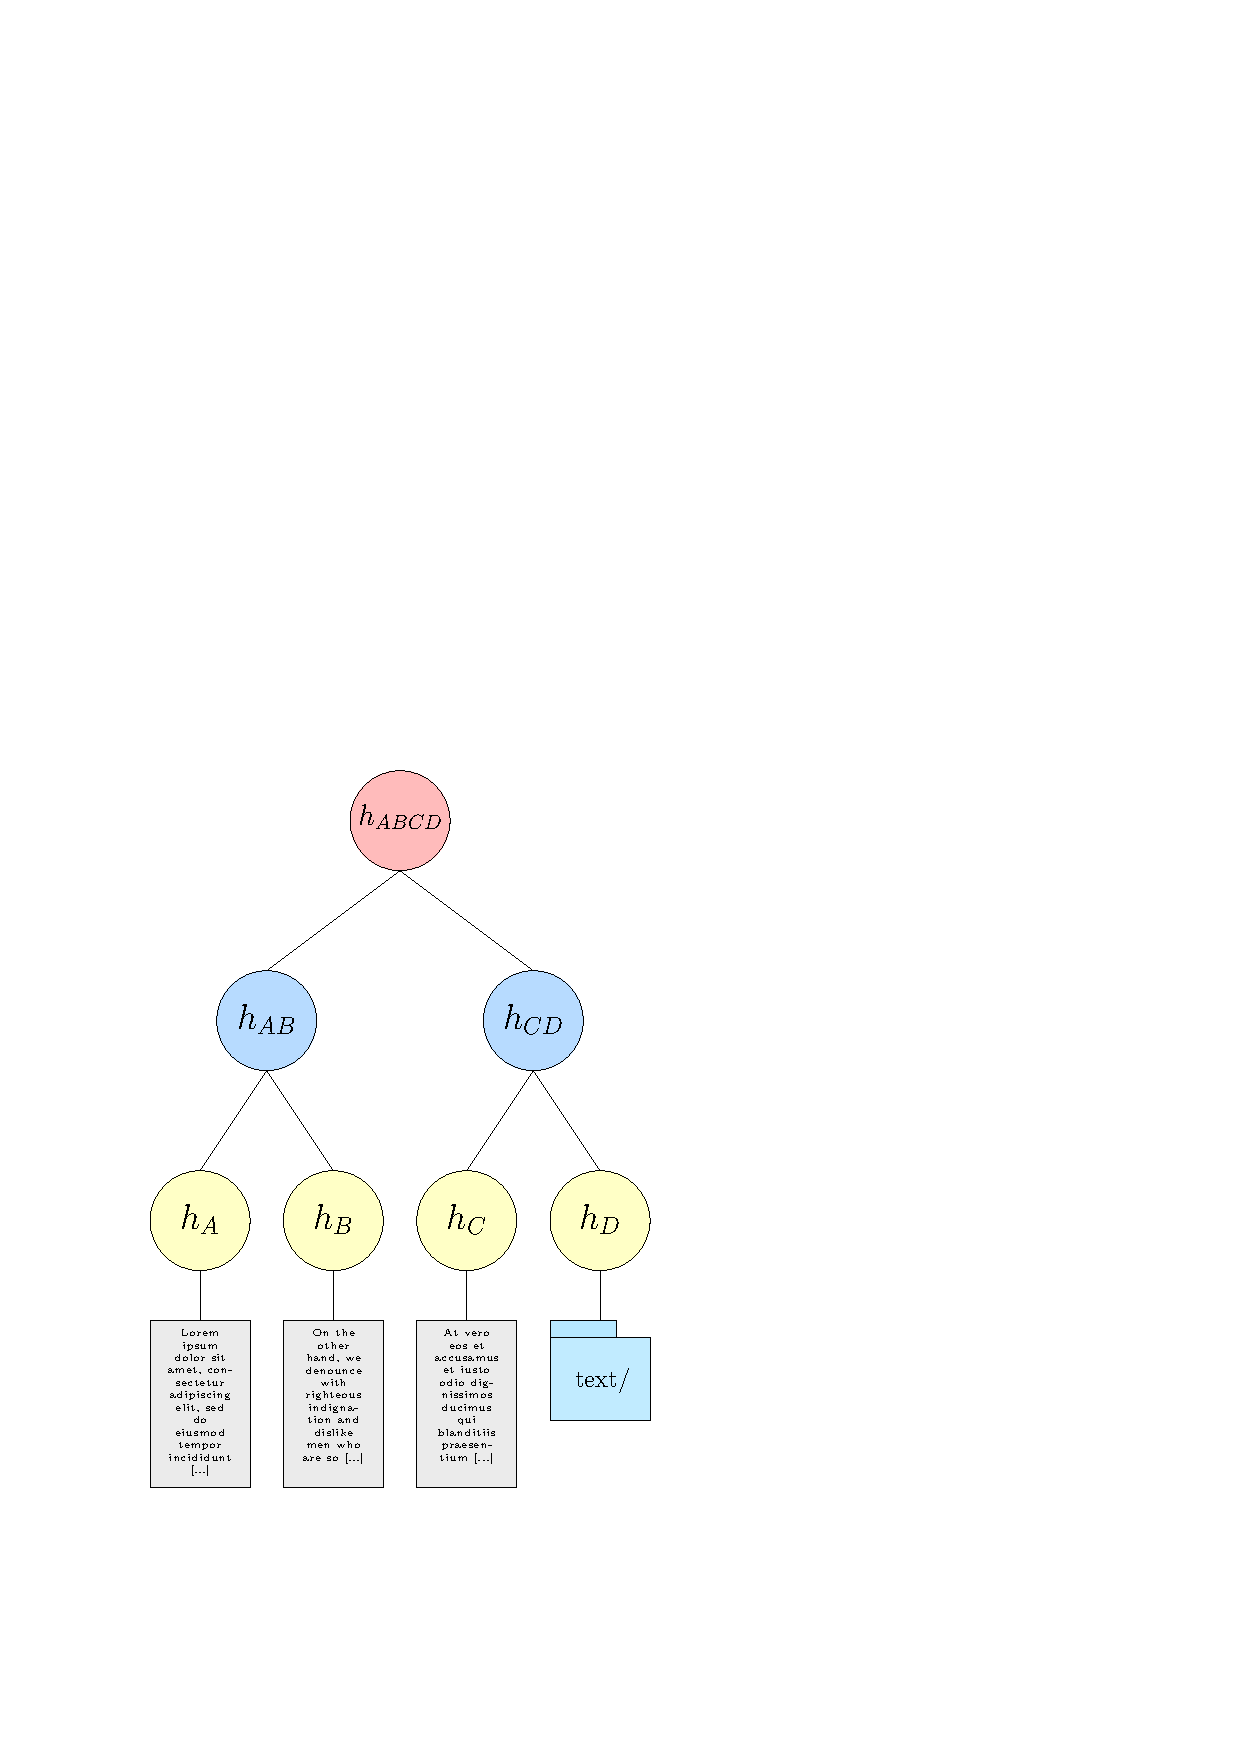
\includegraphics[width=0.4\textwidth]{mt1}
    \end{center}
    \vspace{-20pt}
\end{wrapfigure}
I Merkle Tree sono essenzialmente alberi binari
in cui ogni foglia corrisponde all'hash di uno dei nostri elementi. Risalendo verso la radice ogni
nodo interno calcolerà il proprio hash concatenando gli hash dei nodi figli, infine si avrà
una radice (\textbf{Merkle Root} o MR) il cui hash è univoco a quella lista di elementi che l'albero
ha come foglie, in quella sequenza.
Infatti, utilizzando degli hash generati con una funzione crittografica ``forte", si ha
un'assenza di collisioni tra le Merkle Root.
Perciò sappiamo che, per una determinata sequenza di documenti i cui hash sono le foglie dell'albero, anche solo una
piccola modfica ad un file causerebbe un cambiamento significativo, se non totale, della MR.

Possiamo quindi capire se c'è stato un cambiamento, tuttavia per capire anche
quale dei documenti è stato cambiato bisogna ricorrere al concetto di \textbf{Merkle Proof}.
Per effettuare una verifica tramite Merkle Proof sono tre gli elementi necessari:
\begin{enumerate}
    \item L'elemento (foglia) che vogliamo verificare;
    \item La Merkle Root;
    \item La Merkle Proof, ovvero la lista degli hash dei fratelli lungo il cammino dall'elemento alla radice.
\end{enumerate}
Andando a svolgere questa verifica su ogni documento riusceremo ad individuare i file modificati come
quelli per cui non è possibile ricostruire il cammino verso la radice, lasciando quest'ultima inalterata.

\section{JSON}
\label{sub:json}
Il JavaScript Object Notation (\textbf{JSON})~\cite{json} è un semplice formato per lo scambio di dati,
facile da interpretare e capire sia per i vari linguaggi di programmazione che per gli esseri umani.
Esso, con le librerie apposite per ogni linguaggio, permette un semplice e rapido scambio
di dati tra più applicativi e fornisce metodologie per la conversione di oggetti e collezioni
di dati strutturati in stringhe da salvare in file e viceversa, un'alternativa ragionevole ai database
per applicazioni che cercano di sviluppare architetture distribuite.
Osserviamo e analizziamo un esempio di oggetto JSON:
\begin{lstlisting}[language=json,firstnumber=1]
{ "nome": "Mario",
  "cognome": "Rossi",
  "eta": 27,
  "indirizzo": {
    "indirizzoStradale": "Via Fasulla 123",
    "citta": "Perugia"
  },
  "numeriTelefono": [
    {
      "tipo": "casa",
      "numero": "212 555-1234"
    },
    {
      "tipo": "ufficio",
      "numero": "646 555-4567"
    } ],
  "figli": [],
  "coniuge": null }
\end{lstlisting} 
Possiamo osservare come ogni attributo e il suo valore vengano rappresentati come
\[``key" = value \]
dove il valore è posto tra due virgolette in caso sia una stringa (\textsf{riga 1})
o da nulla in caso sia un tipo primitivo (\textsf{riga 3}).
Un valore può inoltre essere anche un altro oggetto (\textsf{righe 4-7}), in questo caso
vediamo come venga incluso tra parentesi graffe e segua poi al suo interno la sintassi che
abbiamo appena osservato, o un array di valori semplici o oggetti (quest'ultimo alle \textsf{righe 8-16})
andando ad inserire i valori tra parentesi quadre.
È possibile anche rappresentare array vuoti (\textsf{riga 17}), con delle parentesi quadre senza
contenuto, e valori nulli (\textsf{riga 18}) con la parola chiave \textsf{null}.
I valori vengono separati tra loro con una semplice virgola.